%%% fs-state-related - Related work

\label {fs-related-seciton}

Many prior works in the field of stream processing do not consider consistency maintaining as a high priority task. For instance, Aurora~\cite{Abadi:2003:ANM:950481.950485} and Borealis~\cite{abadi2005design} prefer availability and low latency rather than consistency guarantees. Some other works provide only partial consistency. Apache Storm~\cite{apache:storm} supports message tracking mechanism that prevents the loss of data. However, exactly-once semantics is not provided, because duplicates are still possible. Twitter Heron, that was presented as the next generation of Apache Storm~\cite{Kulkarni:2015:THS:2723372.2742788}, does not provide for exactly-once as well. Samza~\cite{Noghabi:2017:SSS:3137765.3137770} also implements fairly similar to Storm model and has the same consistency guarantees.  

One approach to achieve exactly-once semantics is to enforce determinism. As it was mentioned above, if computations are deterministic, it is fairly simple to replay input data in case of failure without producing duplicates, i.e., achieve system-wide idempotence. Micro-batching is a popular approach that combines batch and stream processing. The main idea behind this method is to treat input data as a sequence of small-sized batches. If data items are continuously arriving, they can be packaged into batches at system's entry and then processed in a batch manner. Spark Streaming~\cite{Zaharia:2012:DSE:2342763.2342773} introduces {\it discretized streams} model that is based on micro-batching idea and is unified with Spark's batch processing. Storm Trident~\cite{apache:storm:trident} implements micro-batching on top of Apache Storm. The main advantage of the micro-batching technique is that its properties are naturally derived from batch processing model. Therefore, systems which use this approach are inherently deterministic, fault tolerant and provide strong consistency. However, such systems experience heavy overhead in terms of end-to-end latency, because of the buffering on input.

Another way to provide exactly once semantics is to cope with a non-deterministic model by releasing output items only when the system is ensured that they are consistent and system's restart will not cause releasing duplicates. Apache Flink~\cite{Carbone:2017:SMA:3137765.3137777} uses the variation of Chandy-Lamport algorithm for {\it state snapshotting} mechanism~\cite{2015arXiv150608603C}. This mechanism allows the system to restart processing from certain points. However, because of the non-deterministic computational model, there is a need to take state snapshots and release output items atomically to avoid producing duplicates and the loss of data. To complete this task the adaptation of 2PC protocol for distributed transactions is used. The similar approach for exactly-once processing is applied in IBM Streams~\cite{jacques2016consistent}. The main problem regarding this method is that distributed transactions can provide significant latency overhead because output items cannot be released until the transaction is committed. 

Google's MillWheel~\cite{Akidau:2013:MFS:2536222.2536229} uses a different approach to achieve exactly-once within non-deterministic model. It persistently stores each input item before each operation in order to filter out duplicates if any. Such technique, called {\em strong productions}, makes system idempotent, but provides high overhead on frequent accesses to persistent storage.

The roadmap of approaches for achieving exactly-once and at-least-once guarantees is shown in Figure~\ref{roadmap}. Green elements indicate the path for our approach that is detailed in further sections.

\begin{figure*}[htbp]
  \centering
  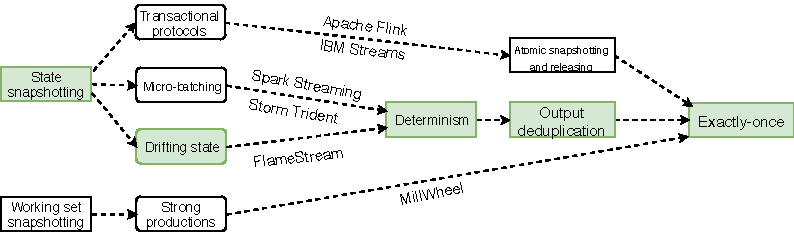
\includegraphics[width=0.97\textwidth]{pics/roadmap}
  \caption{The roadmap of approaches for achieving exactly-once guarantee}
  \label {roadmap}
\end{figure*}



